In \autoref{sec:architectures-biasesgraph} it is discussed, that a pure graph network is independent to the encoding of the problem in e.g. memory.

This is demonstrated in an experiment pictured in \autoref{fig:resiliency-encoding}.
There a CNN and a SGDCF-NNN are studied on the same Ising problem.
In this case the absolute performance is irrelevant, only the relative performance difference resulting from a change to the encoding (random swaps, like described in \autoref{sec:theory-latticepatterns}) will be discussed. 

\begin{figure}[htbp]
    \centering
    \makebox[\textwidth][c]{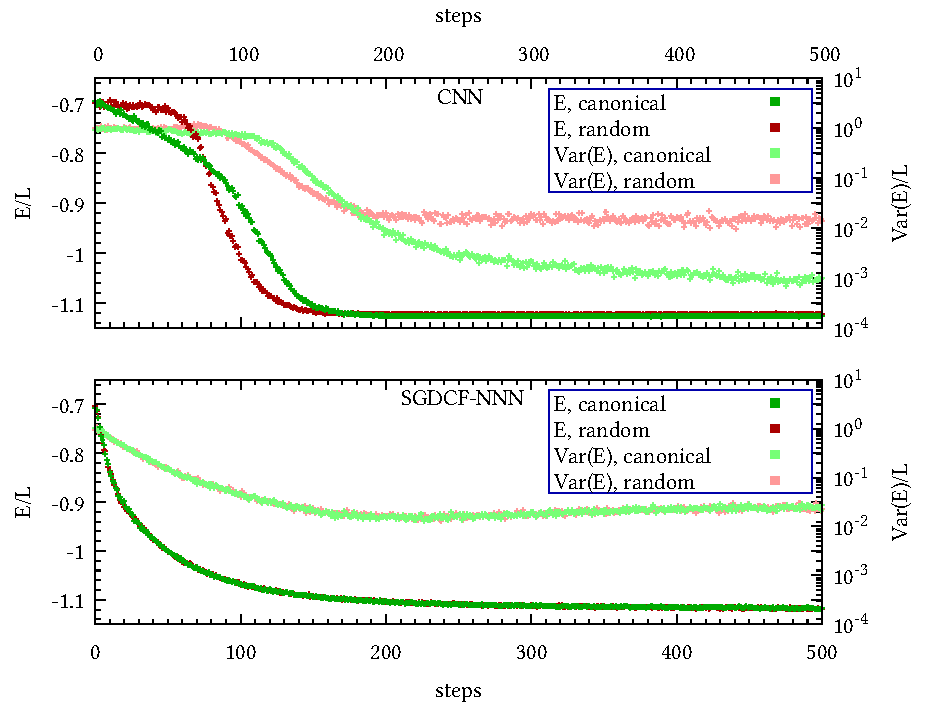
\includegraphics[width=1\textwidth]{./experiments/ground-state-search/resiliency-encoding/encoding-comparison/encoding-comparison.pdf}}
    \caption{
        Visualization of the reaction of a CNN and a SGDCF-NNN network to a change in lattice encoding.
        The calculations are performed for a transverse field Ising model with $J = -1$, $h=-0.7$ on a 1D-linear lattice chain.
        The SGDCF-NNN has a depth of 1, an embed dimension of 16 and a mlp-ratio of 2, making both models have approximately the same number of parameters (CNN: 1280, SGDCF-NNN: 1312).
        The canonical numbering for the lattice sites is printed in green, while the random numbering and therefore unstructured representation in memory is pictured red. 
        The variance is pictured in the same graph, colored in the respective light shade.
    }
    \label{fig:resiliency-encoding}
\end{figure}

The investigated lattice is a linear 1D-chain, therefore the canonical representation of the lattice indicees maps them to a linear array in memory. 
This aligns perfectly with the shape of a 1D convolution, like it is used in the CNN. 
Because of that, the CNN in this case achieves a very high degree of precision (upper green graphs in \autoref{fig:resiliency-encoding}).

Using this relation requires the model to have architectural similarities with the underlying lattice.
This not only requires manual engineering, but may even be very impractical for highly irregular lattices.

Randomizing the lattice indicees shows the CNN's dependency on the canonical structure (upper red graphs in \autoref{fig:resiliency-encoding}).
The variance only converges to a value one magnitude further away from zero.
Instantly indicating the number of weights does no longer suffice to fully parametrize the wavefunction in that ansatz.

In comparison, the SGDCF-NNN - which is a completely graph-based model - receives absolutely no drawback from the encoding change.
The course of the energy and variance are not affected. 
This shows the potential of graph networks to be employed as computational \glqq black boxes\grqq{} that do not need to be engineered to efficiently represent the desired lattice structure, as the adjacency matrix takes care of this automatically.
Furthermore if a good performing network is found, it is more likely to be translatable to related problems.
